\usepackage{tikz}
\usetikzlibrary{decorations.pathreplacing,positioning}

\AtBeginDocument{%
%%% --- PÁGINA 1: CAPA (imagem de capa) ---
\thispagestyle{empty}%
\newgeometry{margin=0pt}%
\mbox{}\vspace*{-\baselineskip}%
\noindent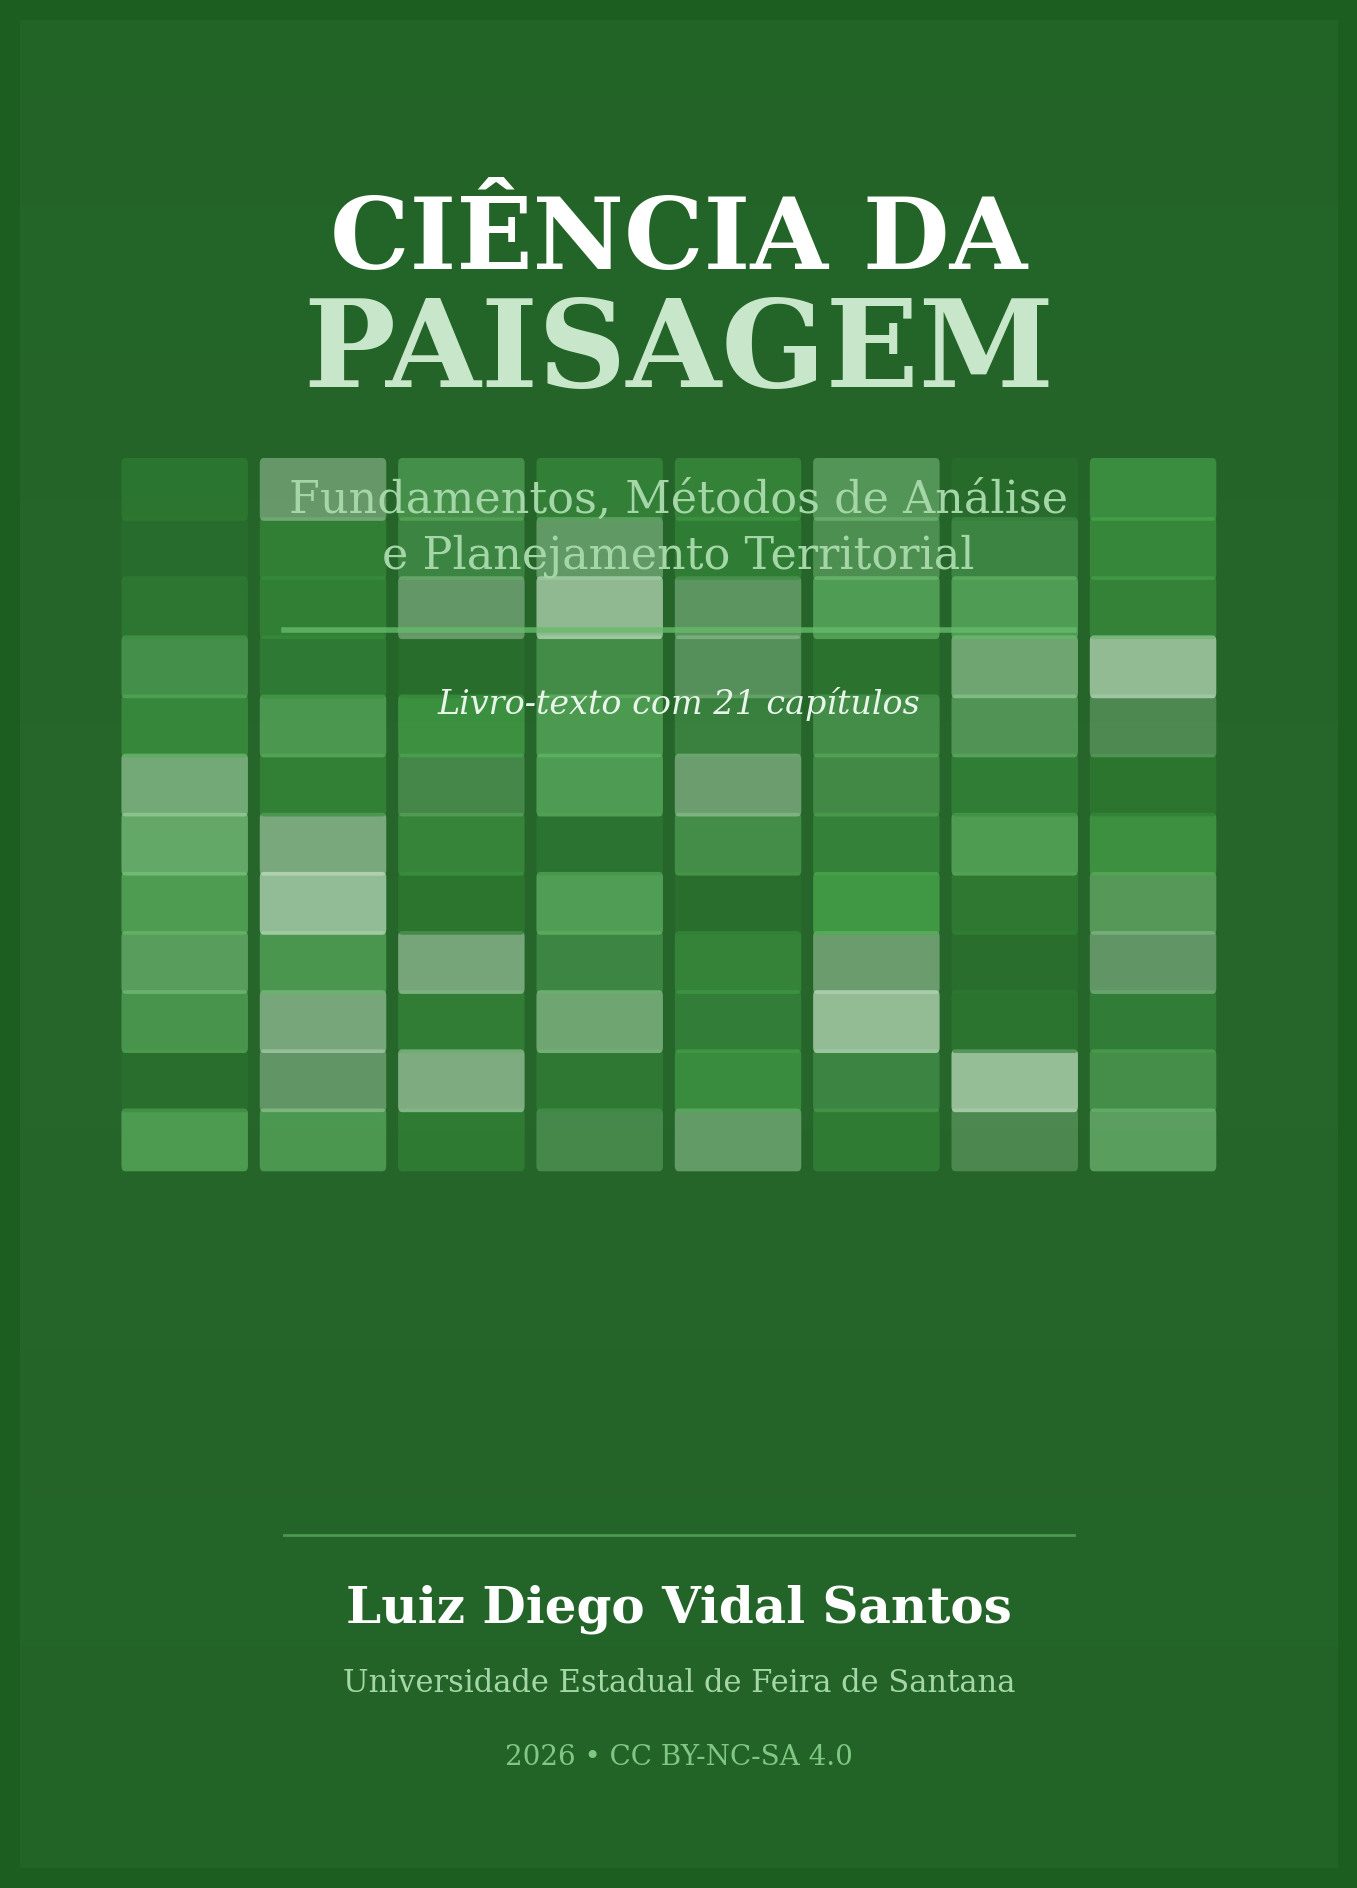
\includegraphics[width=\paperwidth,height=\paperheight]{img/capa_ciencia_paisagem.png}%
\restoregeometry%
\clearpage
%%% --- PÁGINA 2: FOLHA DE ROSTO ---
\thispagestyle{empty}%
\begin{center}
\vspace*{3cm}
{\Large\bfseries Luiz Diego Vidal Santos}\\[2cm]
{\LARGE\bfseries Análise da Paisagem}\\[0.6cm]
{\large Fundamentos, Métodos e Planejamento Territorial}\\[3cm]
{\normalsize 1.\textsuperscript{a} edição}\\[2cm]
{\normalsize Feira de Santana --- BA\\[0.3cm]
Edição do Autor\\[0.3cm]
2026}
\end{center}
\vfill
\clearpage
%%% --- PÁGINA 3: FICHA CATALOGRÁFICA E DADOS EDITORIAIS ---
\thispagestyle{empty}%
\vspace*{\fill}
%% -- Ficha Catalográfica (caixa emoldurada, padrão AACR2) --
\noindent
\begin{center}
\fbox{\parbox{0.85\textwidth}{%
\small
\begin{center}\textbf{Dados Internacionais de Catalogação na Publicação (CIP)}\end{center}
\vspace{4pt}
\hangindent=1.5cm\hangafter=1
Santos, Luiz Diego Vidal.\\
\hspace*{1.5cm}Análise da paisagem: fundamentos, métodos e planejamento territorial / Luiz Diego Vidal Santos. --- 1. ed. --- Feira de Santana, BA: Edição do Autor, 2026.\\[4pt]
\hspace*{1.5cm}Livro digital (PDF/HTML).\\[4pt]
\hspace*{1.5cm}ISBN 978-65-02-02072-2\\[4pt]
\hspace*{1.5cm}DOI: \href{https://doi.org/10.5281/zenodo.19268053}{10.5281/zenodo.19268053}\\[4pt]
\hspace*{1.5cm}1. Análise da paisagem. 2. Planejamento territorial. 3. Ecologia da paisagem. 4. Geoprocessamento. 5. Sensoriamento remoto. I. Título.\\[6pt]
\begin{flushright}CDD 304.2\quad CDU 911.5\end{flushright}
}}
\end{center}

\vspace{1.2cm}

%% -- Dados editoriais --
\noindent\small
\begin{center}
\textbf{Análise da Paisagem: Fundamentos, Métodos e Planejamento Territorial}\\[6pt]
\textcopyright{} 2026, Luiz Diego Vidal Santos.\\
Todos os direitos reservados.\\[10pt]
\textbf{ISBN:} 978-65-02-02072-2\\[6pt]
\textbf{DOI:} \href{https://doi.org/10.5281/zenodo.19268053}{10.5281/zenodo.19268053}\\[6pt]
\textbf{Autor:} Luiz Diego Vidal Santos\\
\textbf{ORCID:} \href{https://orcid.org/0000-0001-8659-8557}{0000-0001-8659-8557}\\[6pt]
\textbf{Afiliação:} Universidade Estadual de Feira de Santana (UEFS)\\
Departamento de Ciências Humanas e Filosofia --- DCHF\\
Feira de Santana, Bahia, Brasil\\[10pt]
\textbf{1.\textsuperscript{a} edição} --- fevereiro de 2026\\[6pt]
Publicação independente (Edição do Autor).\\
Disponível em: \url{https://diegovidalcv.com.br/books/ciencia-paisagem/}\\[10pt]
Este livro é distribuído sob licença\\
\href{https://creativecommons.org/licenses/by-nc-sa/4.0/}{Creative Commons Atribuição-NãoComercial-CompartilhaIgual 4.0 Internacional (CC BY-NC-SA 4.0)}.
\end{center}
\normalsize
\vspace*{\fill}
\clearpage
}
